% !TeX root = ../solution.tex

\hypertarget{he22.04}{%
\chapter{[HE22.04] I Key, You Key, ASCII}\label{he22.04}}

\begin{marginfigure}
	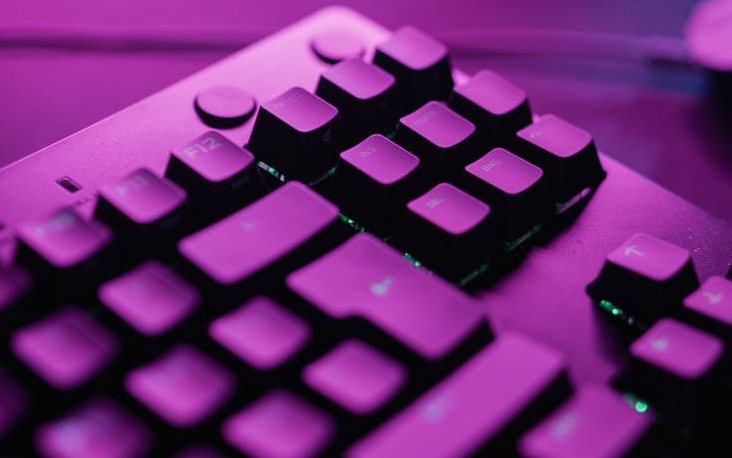
\includegraphics[width=49mm]{level2/challenge4.jpg}
\end{marginfigure}
\subsection{Intro}

Look what I was drawing in my text editor!

\begin{verbatim}
.. .. .. 68 65 32 30 .. .. ..  
.. .. 32 ██ ██ ██ ██ 32 .. ..  
.. 7b ██ ██ ██ ██ ██ ██ 74 ..  
.. 68 ██ ██ ██ ██ ██ ██ 31 ..  
73 ██ ██ ██ ██ ██ ██ ██ ██ 5f  
30 ██ ██ ██ ██ ██ ██ ██ ██ 6e  
33 ██ ██ ██ ██ ██ ██ ██ ██ 5f  
31 ██ ██ ██ ██ ██ ██ ██ ██ 73  
5f ██ ██ ██ ██ ██ ██ ██ ██ 72  
33 ██ ██ ██ ██ ██ ██ ██ ██ 33  
33 ██ ██ ██ ██ ██ ██ ██ ██ 33  
.. 6c ██ ██ ██ ██ ██ ██ 79 ..  
.. 5f ██ ██ ██ ██ ██ ██ 73 ..  
.. .. 31 ██ ██ ██ ██ 6d .. ..  
.. .. .. 70 6c 33 7d .. .. ..  
\end{verbatim}
  

\section{Solution}\label{hv21.04-solution}

Convert the hex numbers to the respective ASCII character:

\noindent\texttt{he2022\{th1s\_0n3\_1s\_r3333ly\_s1mpl3\}}

